\documentclass[10pt,aspectratio=169]{beamer}

% Use the metropolis theme
\usetheme{metropolis}

% Set the color scheme
\usepackage{xcolor}
\definecolor{mDarkTeal}{HTML}{23373b}
\definecolor{mLightBrown}{HTML}{EB811B}
\definecolor{mLightGreen}{HTML}{14B03D}

% Math packages
\usepackage{amsmath}
\usepackage{amssymb}
\usepackage{mathtools}

% Graphics
\usepackage{graphicx}
\usepackage{tikz}

% Additional packages
\usepackage{booktabs}
\usepackage{multicol}

% Title information
\title{F1010 - Modeling with Differential Equations}
\subtitle{Session 1: Course Introduction}
\author{Dr. Juliho Castillo\\julihocc@tec.mx}
\institute{School of Engineering and Sciences\\Academic Department of Sciences}
\date{\today}

\begin{document}

% Title slide
\maketitle

% Table of contents
\begin{frame}{Outline}
    \tableofcontents
\end{frame}

\section{Welcome to F1010}

\begin{frame}{Course Information}
    \begin{itemize}
        \item \textbf{Course Code:} F1010
        \item \textbf{Course Title:} Modeling with Differential Equations
        \item \textbf{Credits:} 3-0-1-5.3-2-30-10-56-16-96-10-2
        \item \textbf{Discipline:} Physics
        \item \textbf{School:} Engineering and Sciences
        \item \textbf{Academic Department:} Sciences
        \item \textbf{Prerequisite:} MA1029
    \end{itemize}
\end{frame}

\begin{frame}{Course Structure}
    \begin{columns}
        \begin{column}{0.5\textwidth}
            \textbf{Session Organization:}
            \begin{itemize}
                \item \textbf{Total Sessions:} 20
                \item \textbf{Duration:} 2 hours each
                \item \textbf{Contact Hours:} 40 hours
            \end{itemize}
        \end{column}
        \begin{column}{0.5\textwidth}
            \textbf{Distribution:}
            \begin{itemize}
                \item 1 opening session
                \item 6 subject modules (3 sessions each)
                \item 1 comprehensive review/exam
            \end{itemize}
        \end{column}
    \end{columns}
\end{frame}

\section{Learning Objectives}

\begin{frame}{What You Will Learn}
    Upon completion of this course, you will be able to:
    
    \begin{enumerate}
        \item \textbf{Define mathematical relations} between relevant physics variables of a system through fundamental principles
        
        \item \textbf{Model the behavior of systems} through equations that describe the system's relevant quantities and rates of change
        
        \item \textbf{Analyze reality based on facts} through inductive-deductive logical reasoning for problem-solving with valid, objective criteria
    \end{enumerate}
\end{frame}

\section{Mathematical Prerequisites}

\begin{frame}{MA1029 Concepts Review}
    \textbf{Essential concepts from your prerequisite course:}
    
    \begin{multicols}{2}
    \begin{itemize}
        \item Functions and their properties
        \item Limits and continuity
        \item Derivatives and differentiation rules
        \item Chain rule applications
        \item Implicit differentiation
        \item Integration techniques
        \item Fundamental Theorem of Calculus
        \item Parametric equations
        \item Polar coordinates
        \item Infinite series
    \end{itemize}
    \end{multicols}
\end{frame}

\begin{frame}{Quick Review: Derivatives}
    \textbf{Basic differentiation rules:}
    
    \begin{align}
        \frac{d}{dx}[x^n] &= nx^{n-1} \\
        \frac{d}{dx}[e^x] &= e^x \\
        \frac{d}{dx}[\sin x] &= \cos x \\
        \frac{d}{dx}[\ln x] &= \frac{1}{x}
    \end{align}
    
    \textbf{Chain Rule:}
    \begin{equation}
        \frac{d}{dx}[f(g(x))] = f'(g(x)) \cdot g'(x)
    \end{equation}
\end{frame}

\section{Introduction to Differential Equations}

\begin{frame}{What is a Differential Equation?}
    \begin{definition}
        A \textbf{differential equation} is an equation that relates a function with one or more of its derivatives.
    \end{definition}
    
    \textbf{Examples:}
    \begin{align}
        \frac{dy}{dx} &= 3x + 2 \quad \text{(First-order)} \\
        \frac{d^2y}{dx^2} + 4y &= 0 \quad \text{(Second-order)} \\
        \frac{\partial u}{\partial t} &= \frac{\partial^2 u}{\partial x^2} \quad \text{(Partial)}
    \end{align}
\end{frame}

\begin{frame}{Physical Significance}
    Differential equations naturally arise in physics and engineering:
    
    \begin{itemize}
        \item \textbf{Newton's Second Law:} $F = ma = m\frac{d^2x}{dt^2}$
        \item \textbf{Radioactive Decay:} $\frac{dN}{dt} = -\lambda N$
        \item \textbf{Population Growth:} $\frac{dP}{dt} = rP$
        \item \textbf{Heat Conduction:} $\frac{\partial T}{\partial t} = \alpha \nabla^2 T$
        \item \textbf{Wave Equation:} $\frac{\partial^2 u}{\partial t^2} = c^2 \frac{\partial^2 u}{\partial x^2}$
    \end{itemize}
    
    \alert{Differential equations are the language of change!}
\end{frame}

\begin{frame}{Classification of Differential Equations}
    \begin{columns}
        \begin{column}{0.5\textwidth}
            \textbf{By Type:}
            \begin{itemize}
                \item Ordinary (ODE)
                \item Partial (PDE)
            \end{itemize}
            
            \textbf{By Order:}
            \begin{itemize}
                \item First-order
                \item Second-order
                \item Higher-order
            \end{itemize}
        \end{column}
        \begin{column}{0.5\textwidth}
            \textbf{By Linearity:}
            \begin{itemize}
                \item Linear
                \item Non-linear
            \end{itemize}
            
            \textbf{By Coefficients:}
            \begin{itemize}
                \item Constant coefficients
                \item Variable coefficients
            \end{itemize}
        \end{column}
    \end{columns}
\end{frame}

\section{Mathematical Modeling}

\begin{frame}{The Modeling Process}
    \begin{center}
        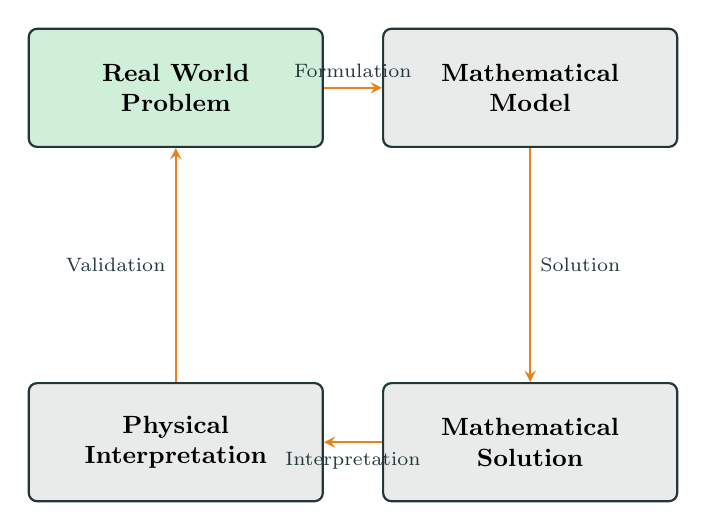
\begin{tikzpicture}[
            node distance=4.5cm, 
            auto,
            box/.style={
                draw, 
                rectangle, 
                rounded corners=3pt,
                text width=3.5cm, 
                text centered,
                minimum height=1.5cm,
                fill=mDarkTeal!10,
                draw=mDarkTeal,
                thick,
                font=\small\bfseries
            },
            arrow/.style={
                ->,
                thick,
                color=mLightBrown,
                >=stealth
            },
            label/.style={
                font=\scriptsize,
                color=mDarkTeal
            }
        ]
            \node (real) [box, fill=mLightGreen!20] {Real World\\Problem};
            \node (math) [box, right of=real] {Mathematical\\Model};
            \node (solution) [box, below of=math] {Mathematical\\Solution};
            \node (interpret) [box, left of=solution] {Physical\\Interpretation};
            
            \draw[arrow] (real) -- (math) node[midway, above, label] {Formulation};
            \draw[arrow] (math) -- (solution) node[midway, right, label] {Solution};
            \draw[arrow] (solution) -- (interpret) node[midway, below, label] {Interpretation};
            \draw[arrow] (interpret) -- (real) node[midway, left, label] {Validation};
        \end{tikzpicture}
    \end{center}
\end{frame}

\begin{frame}{Modeling Principles}
    \textbf{Key steps in mathematical modeling:}
    
    \begin{enumerate}
        \item \textbf{Identify} the variables and parameters
        \item \textbf{Make assumptions} to simplify the problem
        \item \textbf{Formulate} the differential equation
        \item \textbf{Solve} the equation (analytically or numerically)
        \item \textbf{Interpret} the solution in physical terms
        \item \textbf{Validate} against experimental data
        \item \textbf{Refine} the model if necessary
    \end{enumerate}
\end{frame}

\begin{frame}{Example: Population Growth Model}
    \textbf{Problem:} Model the growth of a population over time.
    
    \textbf{Assumptions:}
    \begin{itemize}
        \item Birth rate is proportional to current population
        \item No deaths, immigration, or emigration
        \item Unlimited resources
    \end{itemize}
    
    \textbf{Mathematical Model:}
    \begin{equation}
        \frac{dP}{dt} = rP
    \end{equation}
    
    where $P(t)$ is population at time $t$ and $r$ is the growth rate.
\end{frame}

\section{Course Overview}

\begin{frame}{Module Structure}
    \begin{enumerate}
        \item \textbf{First-Order Differential Equations} (Sessions 2-4)
        \item \textbf{Second-Order Differential Equations} (Sessions 5-7)
        \item \textbf{Power Series Solutions and Special Functions} (Sessions 8-10)
        \item \textbf{Laplace Transform Methods} (Sessions 11-13)
        \item \textbf{Non-Linear Differential Equations} (Sessions 14-16)
        \item \textbf{Partial Differential Equations} (Sessions 17-19)
    \end{enumerate}
    
    \textbf{Final Session:} Comprehensive Review and Assessment (Session 20)
\end{frame}

\begin{frame}{Assessment Framework}
    \begin{itemize}
        \item \textbf{50\% Cumulative Theoretical-Practical Midterm Examinations}
        \begin{itemize}
            \item After modules 2, 4, and 6 (sessions 7, 13, 19)
        \end{itemize}
        
        \item \textbf{20\% Activities, Assignments, and Integrating Cases}
        \begin{itemize}
            \item During practice sessions (4, 7, 10, 13, 16, 19)
        \end{itemize}
        
        \item \textbf{30\% Final Integrating Examination}
        \begin{itemize}
            \item Session 20 (comprehensive assessment)
        \end{itemize}
    \end{itemize}
\end{frame}

\begin{frame}{Required Textbooks}
    \textbf{Primary Text:}
    \begin{itemize}
        \item Nagle, R. Kent. \textit{Fundamentals of Differential Equations and Boundary Value Problems}, 6th ed. Boston: Pearson Education, 2012.
    \end{itemize}
    
    \textbf{Supplementary References:}
    \begin{itemize}
        \item Simmons, George F. \textit{Differential Equations with Applications and Historical Notes}, 2nd ed. New York: McGraw Hill, 1991.
        \item Boyce, W., DiPrima, R., Meade, D. \textit{Elementary Differential Equations}. Wiley, 2016.
    \end{itemize}
\end{frame}

\section{Next Steps}

\begin{frame}{What's Coming Next}
    \textbf{Next Session (Session 2):} First-Order Differential Equations
    
    \textbf{Topics to cover:}
    \begin{itemize}
        \item Linear equations with variable coefficients
        \item Separable equations
        \item Solution techniques and methods
    \end{itemize}
    
    \textbf{Preparation:}
    \begin{itemize}
        \item Review calculus fundamentals
        \item Read Chapter 1 of Nagle textbook
        \item Practice basic integration techniques
    \end{itemize}
\end{frame}

\begin{frame}{Questions and Discussion}
    \begin{center}
        \Huge Questions?
        
        \vspace{1cm}
        
        \large Let's discuss any concerns about the course structure, expectations, or mathematical prerequisites.
    \end{center}
\end{frame}

\begin{frame}[standout]
    Welcome to F1010!\\
    \textbf{Modeling with Differential Equations}
    
    \vspace{1cm}
    
    Ready to explore the mathematics of change?
\end{frame}

\end{document}
